\documentclass[11pt,a4paper]{article}
\usepackage[top=1.00in, bottom=1.0in, left=1.1in, right=1.1in]{geometry}
\usepackage{graphicx}
\usepackage{hyperref}
\usepackage[style=authoryear, backend=biber, natbib = true, style=numeric-comp, sortcites, hyperref, sorting=none, giveninits=true, doi=false,isbn=false,url=false,eprint=false, date=year, maxbibnames = 2, backend=bibtex]{biblatex}
\AtEveryBibitem{\clearfield{pages}}
\AtEveryBibitem{\clearlist{language}}
\AtEveryBibitem{%
  \clearfield{volume}%
  \clearfield{number}}
\AtEveryBibitem{\clearfield{title}}
\renewbibmacro{in:}{}
\usepackage[export]{adjustbox}


\addbibresource{synchrony.bib} 

\begin{document}

\pagenumbering{gobble}

\noindent 
\includegraphics[width=0.5\textwidth, right]{forestry_letterhead.png}

\noindent Dear Dr. Surridge, %emw19Jan -- add name. Also before I forget, I go by EM Wolkovich in publications. 

\vspace{0.25cm} %emw19Jan -- cover letter in very nice shape! I just made major edits to one paragraph; take or leave them. 

\noindent Please consider our paper, entitled ``Solstice optimizes thermal growing season'' for publication as a Brief Communication in \emph{Nature Plants}. 

\vspace{0.25cm}

\noindent Understanding how plants cope with fluctuating climatic conditions has become increasingly important with climate change, across research fields from physiology, ecology, and climatology. Warming has shifted major plant events---leafout, flowering---earlier \supercite{Menzel2006, Fu2019} with potential impacts on growth and, in turn, ecosystem functioning, including carbon storage \supercite{Keenan2014}. These shifts are generally proximately controlled by environmental cues, such as temperature and photoperiod, that plants use to adjust their timing in response to environment variability.

\vspace{0.25cm}
%emw19Jan -- Add Wang citation as suggested below, it hints at how important this work is across plant disciplines.
\noindent Summer solstice has recently been proposed as a universal trigger for key physiological processes \supercite{Zohner2023, Journe2024}, with the potential to redefine how we predict plant responses to climate change. This could also reveal a new fundamental mechanism for how plants sense photoperiod, following on recent advances from molecular biology \supercite{wang2024plants}. Whether plants rely on solstice, however, is highly debated and has highlighted our limited fundamental understanding of the underlying drivers on the timing of plant transitions. 

\vspace{0.25cm}

\noindent Building on these recent findings, we propose a novel test for when plants should optimally transition key physiological processes during the growing season. We use a simple but powerful approach to  examine the thermal energy trade-offs that may drive plant transitions. %emw19Jan -- I feel like you could tack these two previous sentence (or merge into one sentence) onto the end of the last paragraph to lead this paragraph with the below exciting result BUT I also like keeping the background separate from our approach and the title makes the point below so in the end I left this paragraph together. I am just sharing my internal struggle here. 
Averaging across all of Europe, we show that solstice represents a broad-scale optimum, which integrates both environmental predictability (plants ability to anticipate environmental conditions) and growth potential (how much more plants can invest in growth). These results extend over the climates of the Holocene and future climates with continued anthropogenic warming, Yet, our findings also reveal significant variation in the optimal timing across regions, making it difficult to understand how selection would favor solstice as a universal cue, and suggesting future research should equally test for a thermal cue that may allow plants to track growing seasons more accurately.

\vspace{0.25cm}

\noindent Our results bring a new angle to the solstice debate, with implications for both forecasting plant response to global warming and answering fundamental biological questions. We highlight the types of future research that will be needed to disentangle the role of the solstice as a cue for major physiological transitions. Developing a clearer understanding of the optimal drivers of transitions will be critical to better simulate plant timing on a global scale as well as to understand the long-term adaptive responses of plant communities more broadly. 

\vspace{0.25cm}

\noindent Both authors contributed to this work and approve this version for submission. The manuscript is 1535 words, with 19 references and 2 figures, and is not under consideration elsewhere. We hope you find it suitable for publication in \emph{Nature Plants}, and look forward to hearing from you. 

\vspace{0.45cm}
\noindent Sincerely, 
\vspace{0.45cm}\\
\hspace*{-0.5cm}
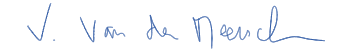
\includegraphics[scale=.65]{sign_long.png} \\
\noindent Victor Van der Meersch, PhD\\
\noindent \emph{Forest \& Conservation Sciences}\\
\noindent \emph{University of British Columbia}

\clearpage

\paragraph{References}
\printbibliography[heading=none]


\newpage

\end{document}


